\hypertarget{problems}{%
\section{Problems}\label{problems}}

\begin{enumerate}
\item
  What is the difference between accuracy and resolution?
\item
  What is meant by serial chain manipulator and how is this different
  from a parallel chain manipulator?
\item
  What is meant by cartesian and cylindrical robot designs? Why would
  you select one over the otehr?
\item
  What mechanical property do the ball screw, threaded rod and rack \&
  pinon share?
\item
  Define configuration space and workspace. What mathematical object
  relates them?
\item
  What is meant by forward position kinematics? What is meant by inverse
  velocity kinematics?
\item
  Graph the workspace of a two-link manipulator centered at the origin
  with \(a_1 = 15\) and \(a_2 = 10\).
\item
  Assume that you have a two link planar manipulator. \(\theta_1\) is
  the angle between the x axis (measured counter-clockwise as positive)
  and the first link arm. \(\theta_2\) is the angle between the second
  link arm and the first link arm (again measured counter-clockwise as
  positive). The link lengths are \(a_1, a_2\). Derive the formulas for
  \(dx/dt\) and \(dy/dt\) as a function of \(d\theta_1/dt\) and
  \(d\theta_2/dt\).
\item
  Using the two link planar manipulator described in the previous
  problem. Derive the formulas for \(d\theta_1/dt\) and \(d\theta_2/dt\)
  as a function of \(x, y\), \(dx/dt\) and \(dy/dt\).
\item
  Given the two link manipulator as described in the previous problems
  with the length of the first link \(a_1 = 10\) and the second link
  \(a_2 = 10\).

  \begin{enumerate}
  \def\labelenumii{\alph{enumii}.}
  \tightlist
  \item
    If \(\theta_1 = 45^\circ\), \(\theta_2 = 45^\circ\), find \(x\) and
    \(y\).
  \item
    If \(\theta_1 = 45^\circ\), \(\theta_2 = 45^\circ\),
    \(d\theta_1/dt = 5^\circ s^{-1}\),
    \(d\theta_2/dt = 10^\circ s^{-1}\) find \(dx/dt\) and \(dy/dt\).
  \end{enumerate}
\item
  Given the two link manipulator as above with the length of the first
  link \(a_1 = 10\) and the second link \(a_2 = 10\).

  \begin{enumerate}
  \tightlist
  \item
    If \(x = 12\), \(y = 14\), find \(\theta_1\) and \(\theta_2\)
  \item
    If \(x = 12\), \(y = 14\), \(dx/dt = -0.25\), \(dy/dt = 0.5\), find
    \(d\theta_1/dt\) and \(d\theta_2/dt\)
  \end{enumerate}
\item
  Assume that you have a two link planar manipulator. \(\theta_1\) is
  the angle between the x axis (measured clockwise as positive) and the
  first link arm. \(\theta_2\) is the angle between the second link arm
  and the first link arm (again measured clockwise as positive). Due to
  servo limitations: \(-100^\circ < \theta_1 < 100^\circ\),
  \(-150^\circ < \theta_2 < 150^\circ\). Also assume the first link is
  20cm long and the second link is 15cm.

  \begin{enumerate}
  \def\labelenumii{\alph{enumii}.}
  \tightlist
  \item
    What is the configuration space?
  \item
    What is the workspace?
  \end{enumerate}
\item
  Find the forward velocity kinematics equations for the two link
  manipulator.
\item
  Assume that you have a two link manipulator that is operating in the
  vertical plane, meaning the two arms lie in the
  \(x-z`plane. Attach the base to a rotational joint so the
  arm rotates around the :math:`z\) axis. Assume the base joint does not
  induce an offset distance \emph{d}. See \texttt{fig:two-link-z} .

  \leavevmode\hypertarget{fig:two-link-z}{}%
  \begin{figure}
  \centering
  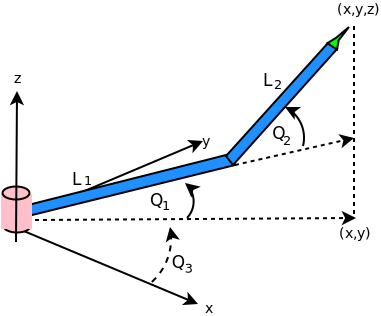
\includegraphics[width=0.5\textwidth,height=\textheight]{TermsFigures/twolinkalt2.*}
  \caption{Two link manipulator.}
  \end{figure}

  \begin{enumerate}
  \def\labelenumii{\alph{enumii}.}
  \tightlist
  \item
    Find the position of the end effector as a function of joint angles.
  \item
    Find the inverse kinematic formula.
  \end{enumerate}
\item
  Typos can creep up in textbooks, papers and reference materials. How
  would test the accuracy of the formulas given in equations
  \texttt{paralleltwolinkforward} and \texttt{paralleltwolinkIK}?
  Discuss.
\item
  Find the forward velocity kinematics equations for the parallel two
  link manipulator.
\item
  Derive the formula for \texttt{paralleltwolinkforward}:

  \[(x,y) = \left( \frac{a+c}{2} + \frac{v (b-d)}{u} , \frac{b+d}{2} + \frac{v (c-a)}{u} \right)\]

  Hint: define the segment from \((a,b)\) to \((c,d)\) as \(B\) (the
  base of the triangle), and \(\vec{A}\) as a vector which is a
  perpendicular to \(B\), see \texttt{Fig:paralleltwolink3} .

  \leavevmode\hypertarget{Fig:paralleltwolink3}{}%
  \begin{figure}
  \centering
  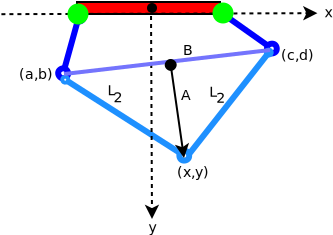
\includegraphics[width=0.4\textwidth,height=\textheight]{TermsFigures/2dDelta3.png}
  \caption{Extraction of the isosceles triangle.}
  \end{figure}
\item
  Derive the formulas for the parallel two link manipulator inverse
  kinematics given in \texttt{paralleltwolinkIK}. Hint:
  \texttt{Fig:paralleltwolinkIK}.

  \leavevmode\hypertarget{Fig:paralleltwolinkIK}{}%
  \begin{figure}
  \centering
  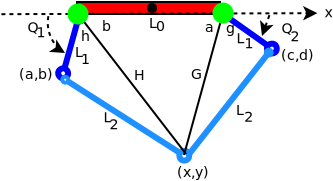
\includegraphics[width=0.4\textwidth,height=\textheight]{TermsFigures/2dDelta4.png}
  \caption{Parallel Two Link Inverse Kinematics variables}
  \end{figure}
\item
  The Denavit-Hartenberg link definition contains rotation matrices,
  \(R\), and translation matrices, \(T\), in homogeneous coordinates.
  Which pairs of matrices commute and which do not. For example, is
  \(RT = TR\)?. Is \(T_1T_2 = T_2T_1\)?
\item
  Translate the following DH parameters into a DH convention
  transformation matrix.

  \begin{longtable}[]{@{}lllll@{}}
  \toprule
  \begin{minipage}[b]{0.08\columnwidth}\raggedright
  Link\strut
  \end{minipage} & \begin{minipage}[b]{0.23\columnwidth}\raggedright
  \(\theta\)\strut
  \end{minipage} & \begin{minipage}[b]{0.14\columnwidth}\raggedright
  \(d\)\strut
  \end{minipage} & \begin{minipage}[b]{0.17\columnwidth}\raggedright
  \(a\)\strut
  \end{minipage} & \begin{minipage}[b]{0.23\columnwidth}\raggedright
  \(\alpha\)\strut
  \end{minipage}\tabularnewline
  \midrule
  \endhead
  \begin{minipage}[t]{0.08\columnwidth}\raggedright
  1\strut
  \end{minipage} & \begin{minipage}[t]{0.23\columnwidth}\raggedright
  \(\theta_1\)\strut
  \end{minipage} & \begin{minipage}[t]{0.14\columnwidth}\raggedright
  1.0\strut
  \end{minipage} & \begin{minipage}[t]{0.17\columnwidth}\raggedright
  \(a_1\)\strut
  \end{minipage} & \begin{minipage}[t]{0.23\columnwidth}\raggedright
  0\strut
  \end{minipage}\tabularnewline
  \begin{minipage}[t]{0.08\columnwidth}\raggedright
  2\strut
  \end{minipage} & \begin{minipage}[t]{0.23\columnwidth}\raggedright
  0\strut
  \end{minipage} & \begin{minipage}[t]{0.14\columnwidth}\raggedright
  0\strut
  \end{minipage} & \begin{minipage}[t]{0.17\columnwidth}\raggedright
  \(a_2\)\strut
  \end{minipage} & \begin{minipage}[t]{0.23\columnwidth}\raggedright
  \(45^\circ\)\strut
  \end{minipage}\tabularnewline
  \bottomrule
  \end{longtable}
\item
  Modify the robot arm found in \texttt{fig:two-link-z} where the base
  joint raises the arm by \(d_1\) in the \emph{z} direction. When the
  base joint angle is zero, \(\theta_1=0\), the two link arms indicated
  by \(a_2, a_3\) lie in the x-z plane. The latter two joints would have
  an axis of rotation parallel to the y axis (again when
  \(\theta_1=0\)).

  \begin{enumerate}
  \tightlist
  \item
    What is the DH parameter table?
  \item
    Write out the DH transformation matrices.
  \item
    Find the forward kinematics.
  \end{enumerate}

  \leavevmode\hypertarget{Fig:offsetplanar1}{}%
  \begin{figure}
  \centering
  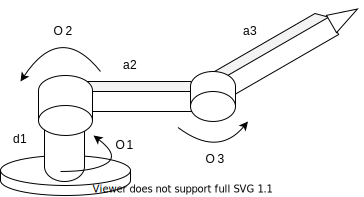
\includegraphics[width=0.5\textwidth,height=\textheight]{TermsFigures/offsetplanar1.*}
  \caption{Offset Two Link}
  \end{figure}
\item
  Modify the robot arm found in \texttt{fig:two-link-z} where the base
  joint raises the arm by \(d_1\) in the \emph{z} direction. In adition,
  the joint mounts the arm along the rotation direction by \(a_1\). When
  the base joint angle is zero, \(\theta_1=0\), the two link arms
  indicated by \(a_2, a_3\) lie in the x-z plane. The latter two joints
  would have an axis of rotation parallel to the y axis (again when
  \(\theta_1=0\)).

  \begin{enumerate}
  \tightlist
  \item
    What is the DH parameter table?
  \item
    Write out the DH transformation matrices.
  \item
    Find the forward kinematics.
  \end{enumerate}

  \leavevmode\hypertarget{Fig:offsetplanar2}{}%
  \begin{figure}
  \centering
  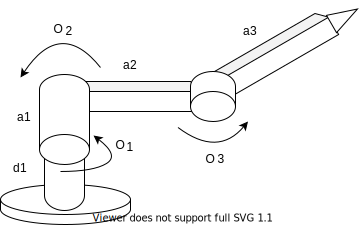
\includegraphics[width=0.5\textwidth,height=\textheight]{TermsFigures/offsetplanar2.*}
  \caption{Offset Two Link with side mount}
  \end{figure}
\item
  For the robotic arm found in \texttt{Fig:offsetplanar3}, the distance
  \(d_1\) is constant where \(a_2, a_3\) can vary.

  \begin{enumerate}
  \tightlist
  \item
    What is the DH parameter table?
  \item
    Write out the DH transformation matrices.
  \item
    Find the forward kinematics.
  \item
    Compare your DH convention approach to a direct trigonometric
    method.
  \end{enumerate}

  \leavevmode\hypertarget{Fig:offsetplanar3}{}%
  \begin{figure}
  \centering
  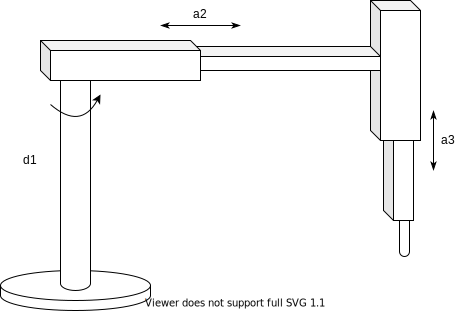
\includegraphics[width=0.5\textwidth,height=\textheight]{TermsFigures/offsetplanar3.*}
  \caption{Cylindrical robot.}
  \end{figure}
\item
  Assume that your differential drive robot has 10 cm diameter wheels
  and a total axle length (wheel to wheel) of 20 cms. If both wheels are
  turning at 0.8 revolutions per second, what is the speed of the robot.
\item
  Using the same robot as previous problem, but where the left wheel is
  turning at 1.5 radians per second and the right wheel is turning at
  1.8 radians per second. Determine the linear velocity and path of the
  robot. You may assume the initial pose is (0,0,0) at \(t=0\).
\item
  For the differential drive robot, let \(r=10\), \(L=15\),
  \(\dot{\phi_1} = 0.9\) \(\dot{\phi_2}= 1.2\).

  \begin{enumerate}
  \def\labelenumii{\alph{enumii}.}
  \tightlist
  \item
    What is the angular velocity of the robot?
  \item
    What is the velocity vector for the robot when
    \(\theta = 45^\circ\)?
  \end{enumerate}
\item
  Let \(r=10\), \(L=15\). If you program the robot to drive straight and
  the robot traces out a circle of diameter 3 meters while traveling 1
  m/s, what are the two wheel speeds?
\item
  Say you have a differential drive robot that has an axle length of
  30cm and wheel diameter of 10cm. Find the angular velocity for the
  left and right wheel if the robot is going to

  \begin{enumerate}
  \def\labelenumii{\alph{enumii}.}
  \tightlist
  \item
    Spin in place at a rate of 6 rpm (revolutions per min),
  \item
    Drive a circle of radius 1 meter (measured center of circle to
    middle of axle) at 3 rpm,
  \item
    Drive a straight line at 1 meter / min.
  \end{enumerate}
\item
  Given a differential drive robot starting from (0,0,0) find the final
  position when wheel velocities are given by:\\
  t=0 to t=5: \(\omega_1\) = 2, \(\omega_2\) = 2\\
  t=5 to t=6: \(\omega_1\) = 3, \(\omega_2\) = 4\\
  t=6 to t=10: \(\omega_1\) = 1, \(\omega_2\) = 2\\
  where D=10, L=16.
\item
  List the variables in the configuration space of a circular ground
  robot that can drive around and use a telescopic arm with a rotational
  base, lifting servo and elbow joint servo.
\end{enumerate}
